% Auto-generated figure includes — paste into LaTeX sections

% Figure 2: Main results bar chart
\begin{figure}[t]
\centering
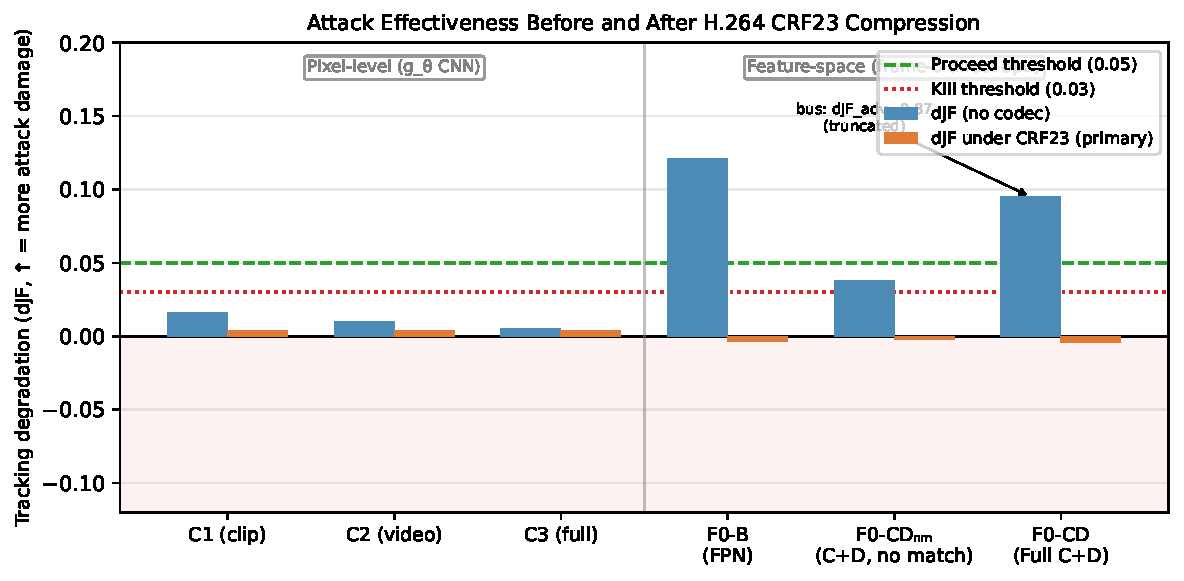
\includegraphics[width=\linewidth]{../figures/fig2_main_results.pdf}
\caption{Tracking degradation (dJF) before and after H.264 CRF23 compression across all six experiments. Blue bars: attack effectiveness without codec; orange bars: dJF under CRF23 (primary metric). Dashed lines mark the proceed (0.05) and kill (0.03) thresholds. All orange bars fall below the kill threshold.}
\label{fig:main_results}
\end{figure}

% Figure 4: Per-video scatter
\begin{figure}[t]
\centering
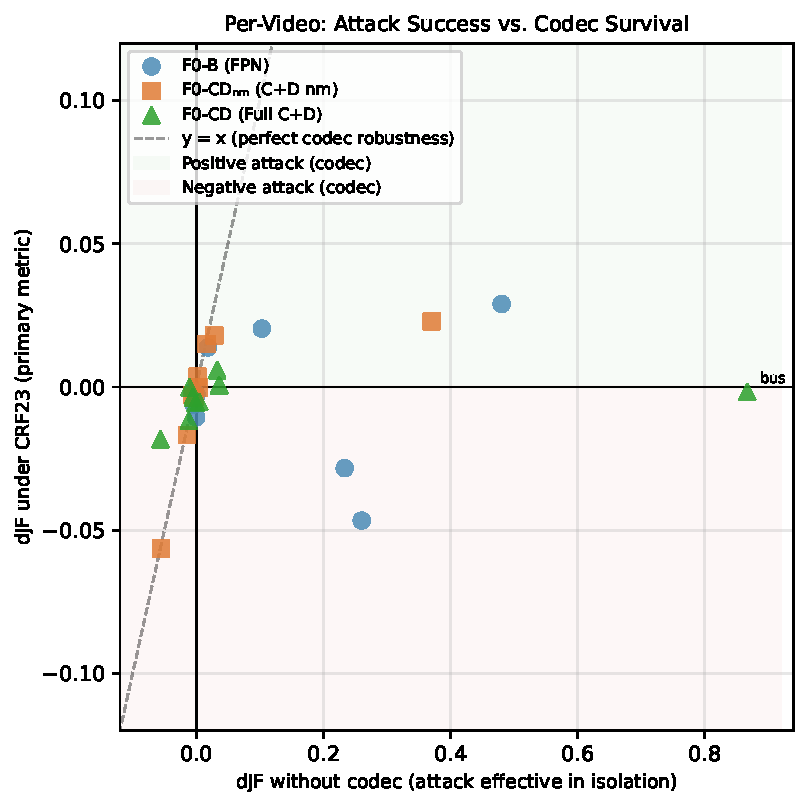
\includegraphics[width=0.85\linewidth]{../figures/fig4_scatter.pdf}
\caption{Per-video dJF without codec (x-axis) vs.\ dJF under CRF23 (y-axis) for the three feature-space attack modes (27 data points). A perfectly codec-robust attack would lie on $y=x$ (dashed line). All attacks collapse toward $y=0$ regardless of insertion point. The bus video (F0-CD, $x=0.87$) dramatically illustrates that optimizer success does not imply codec survival.}
\label{fig:scatter}
\end{figure}
